% GBFS Audit Catalogue --- Computer Standards & Interfaces submission draft
% Reformatted from the Patterns (Cell Press) draft (gold_standard_patterns.tex)
% for Elsevier Computer Standards & Interfaces author guidelines :
%   - <=250 word abstract
%   - 3-5 highlights, each <=85 characters
%   - 1-7 keywords
%   - numbered sections (1, 1.1, ...)
%   - numbered references [1] (style: unsrt)
%   - CRediT author contributions
%   - explicit declarations of interests / generative AI use
%   - data availability statement

\documentclass[11pt,a4paper]{article}

\usepackage[T1]{fontenc}
\usepackage[utf8]{inputenc}
\usepackage{lmodern}
\usepackage[margin=2.5cm]{geometry}
\usepackage{microtype}
\usepackage{amssymb,amsmath,amstext}
\usepackage{booktabs}
\usepackage{graphicx}
\graphicspath{{figures/}}
\usepackage{algorithm2e}
\usepackage{xcolor}
\usepackage{url}
\usepackage[colorlinks=true,linkcolor=blue,citecolor=blue,urlcolor=blue]{hyperref}
\usepackage{enumitem}
\usepackage{caption}
\usepackage{titlesec}
\usepackage{authblk}

\titleformat{\section}{\large\bfseries\sffamily\color{black!85}}{\thesection}{0.8em}{}
\titleformat{\subsection}{\normalsize\bfseries\sffamily\color{black!75}}{\thesubsection}{0.8em}{}

\newcommand{\ie}{\emph{i.e.}}
\newcommand{\eg}{\emph{e.g.}}
\newcommand{\etc}{etc.}

\newenvironment{highlights}{%
  \par\noindent\textsf{\bfseries\large Highlights}\par\smallskip
  \begin{itemize}[leftmargin=1.4em,itemsep=0.15em,topsep=0.2em]}{%
  \end{itemize}\par\medskip}

\title{\bfseries\sffamily\Large Auditing GBFS bike-sharing feeds at country and global scale:\\
A reproducible anomaly taxonomy for open mobility data}

\author[1]{Rohan Foss\'e\thanks{Lead contact: \texttt{rfosse@cesi.fr}}}
\author[2]{Ga\"el Pallares}
\affil[1]{CESI Engineering School, Montpellier, France}
\affil[2]{CESI LINEACT (EA 7527), Montpellier, France}
\date{}

\begin{document}
\maketitle

% Graphical abstract: per Elsevier CSI author guidelines the graphical
% abstract is uploaded as a separate file via Editorial Manager and is
% NOT embedded in the manuscript PDF. The file `fig00_visual_abstract.png`
% in `figures/` is the production asset to upload at submission time.
% (Comment the block below in/out for working drafts vs. final submission.)
%
% \begin{figure}[!t]
% \centering
% 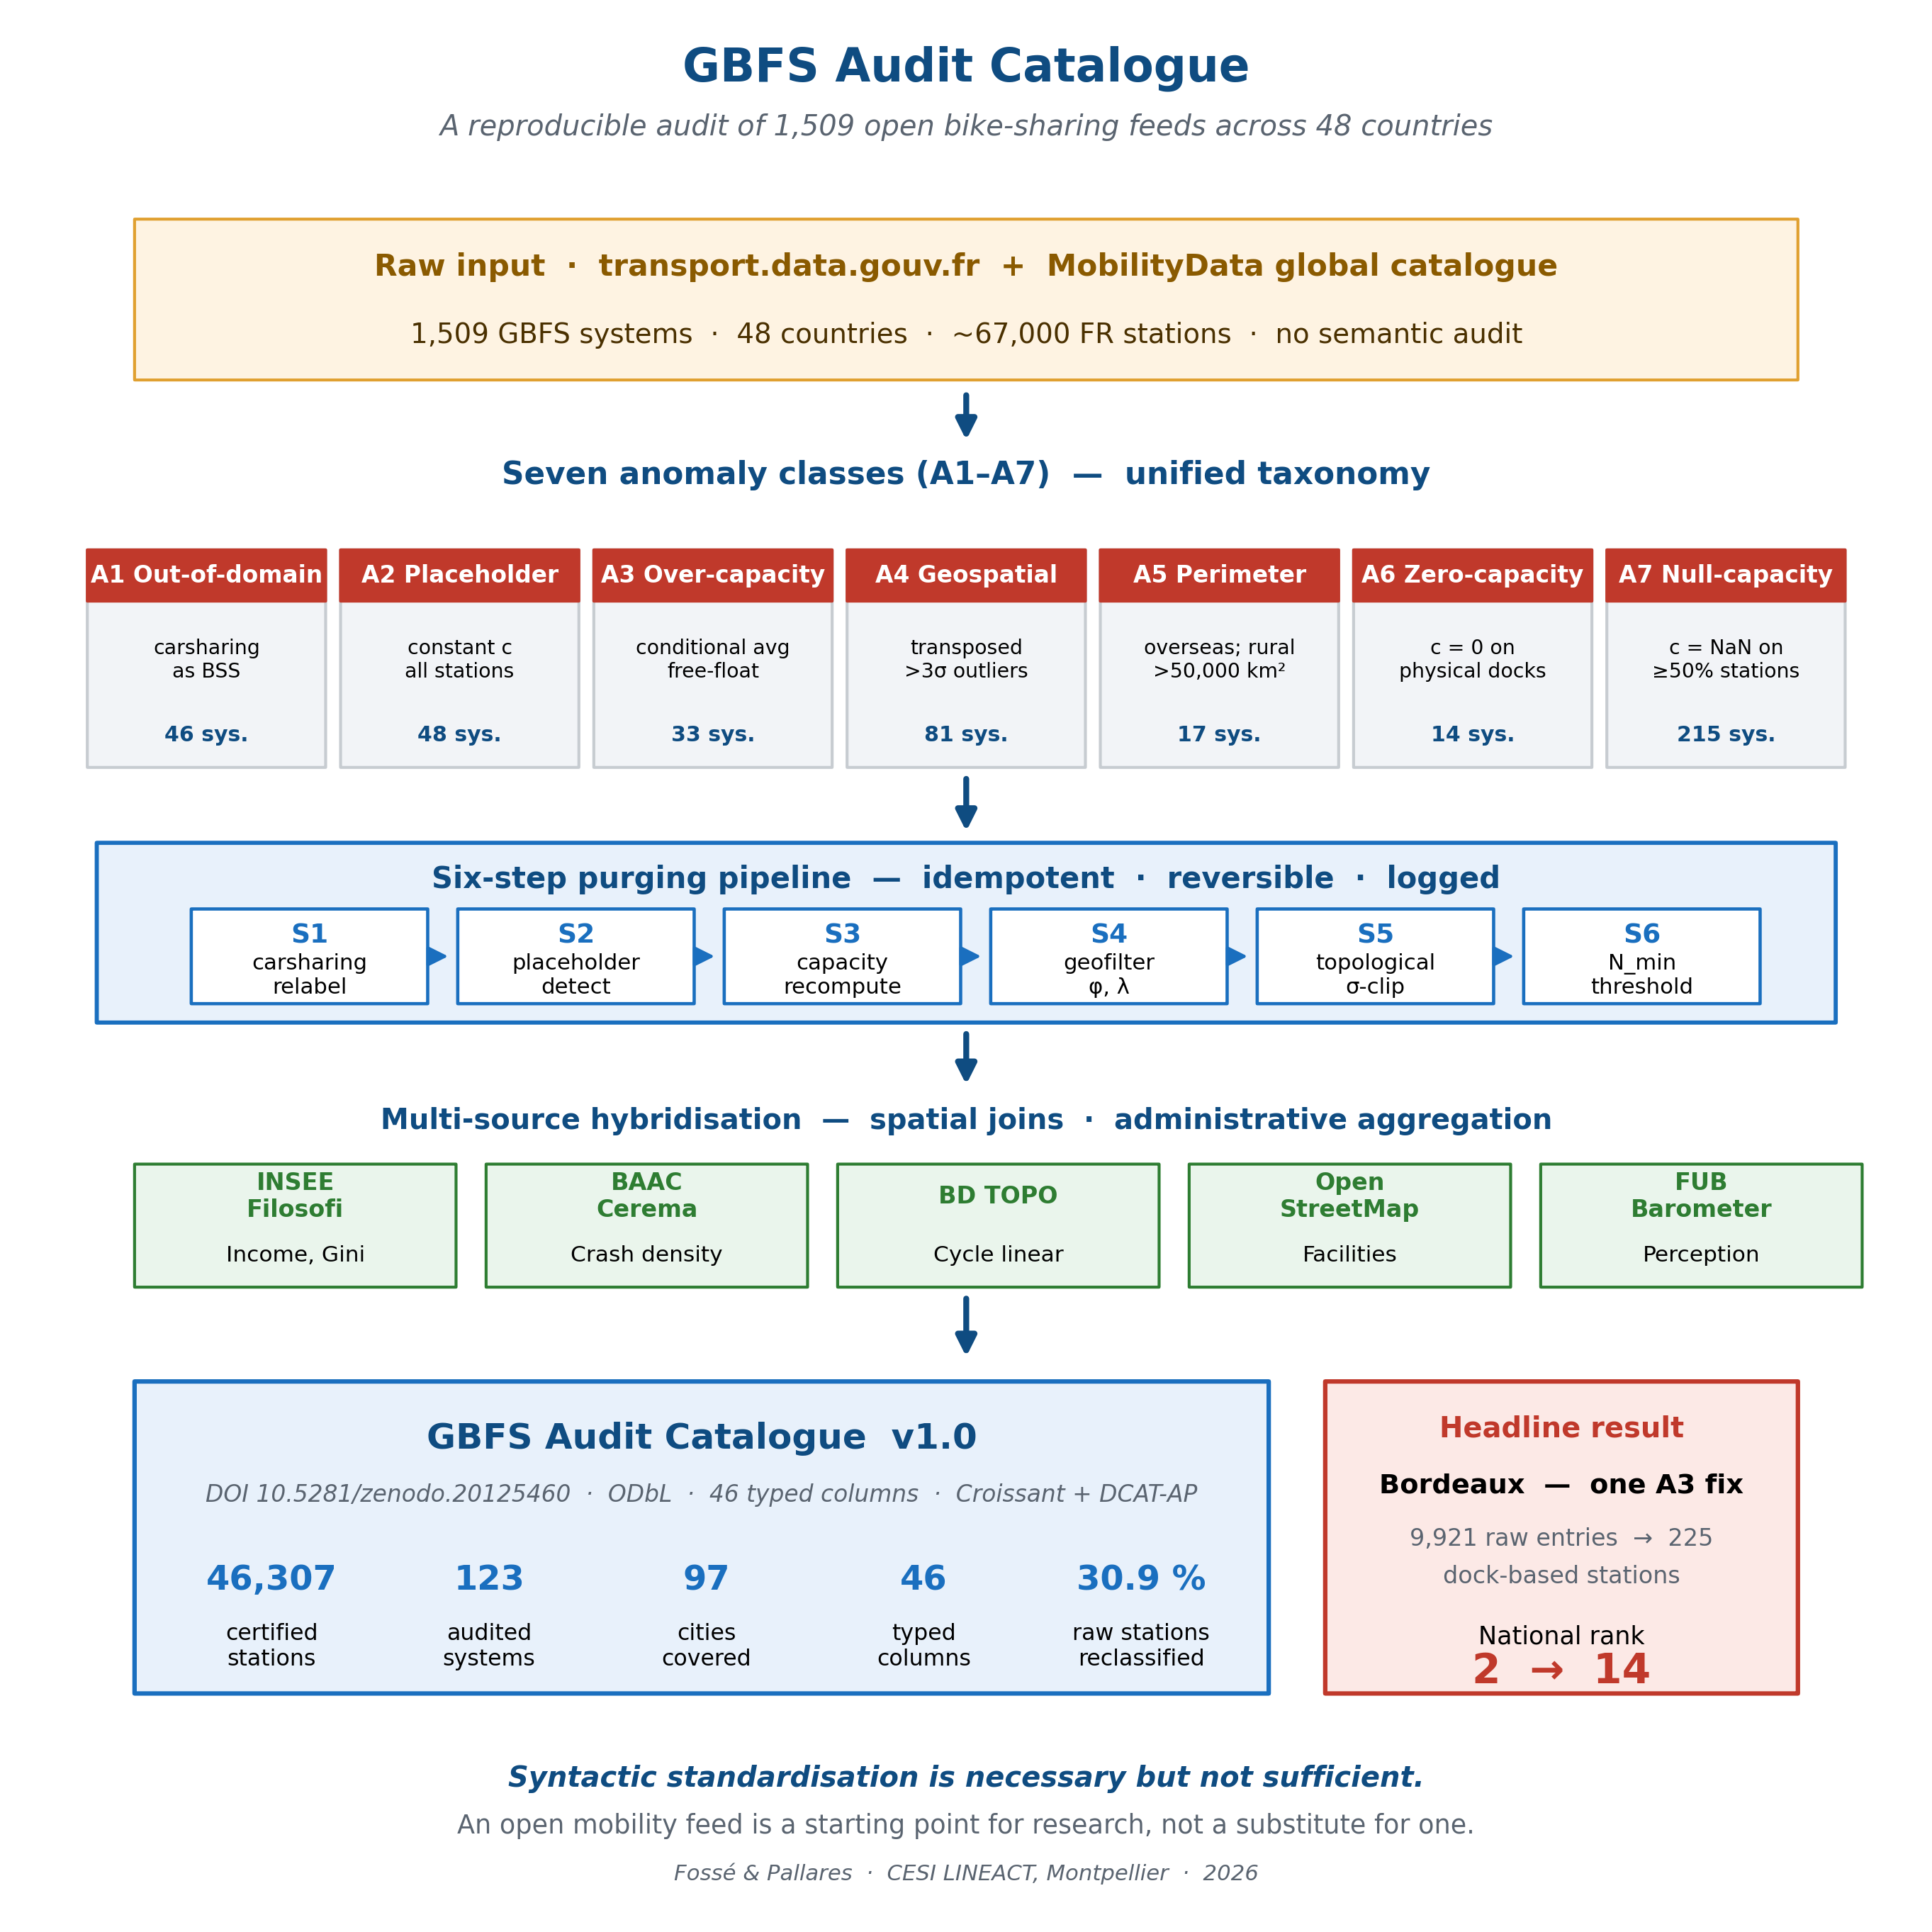
\includegraphics[width=0.85\linewidth]{fig00_visual_abstract.png}
% \caption*{}
% \end{figure}

\section*{Abstract}
\noindent
Open mobility feeds are increasingly assumed to be directly ingestible
into quantitative research pipelines: the General Bikeshare Feed
Specification (GBFS) is now a regulatory requirement for French
operators and is catalogued worldwide by MobilityData. We show that
this syntactic standardisation is necessary but not sufficient. An
audit of the 123 French GBFS systems combined with an exhaustive
sweep of the MobilityData canonical catalogue (1{,}509 systems
across 48 countries) yields a unified taxonomy of seven anomaly
classes (A1--A7) covering out-of-domain inclusion, placeholder
capacity, structural over-capacity, geospatial error,
out-of-perimeter coverage, zero-capacity dock, and null
capacity field. Across the French corpus the taxonomy
reclassifies \textbf{30.9\,\%} of the raw stations (95\,\%
bootstrap CI [30.5, 31.3]); across the global catalogue it flags
204 systems on A1--A5, 14 on A6 and 215 on A7, jointly covering
70{,}176 stations on A7 alone. We formalise a six-step idempotent
purging protocol and release the resulting \emph{GBFS Audit
Catalogue} (46{,}307 stations, 97 cities) on Zenodo. The Czech Republic is the European
hotspot (55.6\,\% of audited systems flagged, all from a single
operator, mirroring \emph{Pony} in France). A positive control on
Beryl London shows the standard can be used correctly when an audit
tier exists. A single A3 correction moves Bordeaux from rank 2 to
rank 14 in a soft-mobility ranking, quantifying the policy cost of
skipping the audit. The dataset, pipeline and Docker image are
released for bit-exact reproduction.

\begin{highlights}
\item Audit of 1{,}509 GBFS systems worldwide; unified taxonomy of 7 anomaly classes
\item Hotspots are operator-driven: nextbike (Czechia), Pony (France)
\item Single GBFS capacity field carries 6 incompatible semantics in the FR corpus
\item 30.9\,\% of raw FR stations reclassified after the six-step purging protocol
\item Audit Catalogue (46k stations) FAIR-released, code and Docker reproducible
\end{highlights}

\noindent\textbf{Keywords:} GBFS; data quality; open mobility data; FAIR; reproducibility; bike sharing; standards compliance.

% ===================================================================
\section{Introduction}

For more than a decade, bike-sharing systems have been a structural
component of urban mobility policy in France and across Europe, advancing
goals of liveability, decarbonisation and last-kilometre integration. To
support inter-operability of the resulting fleets, the General Bikeshare
Feed Specification (GBFS), introduced by the North American Bikeshare
Association in 2015 and now maintained by the Open Mobility Foundation,
provides a shared ontology covering station geolocation, dock counts,
real-time availability and pricing
\cite{Mobi2024,OMF2023}. In France, the 2019 Mobility Orientation Law
(LOM, article L.~1115-1 of the transport code) makes the publication of
these feeds on \emph{transport.data.gouv.fr} a regulatory acquis, so
that by 2026 the working assumption of many research and policy
pipelines is that GBFS feeds can be ingested directly.

That working assumption is misleading. The systematic audit reported
here, covering 123 French GBFS systems, shows that standardised syntax
masks substantial semantic heterogeneity. Three findings make the gap
concrete. First, the same field
(\texttt{station\_information.capacity}) covers radically different
realities: a physical dock count for dock-based fleets, a theoretical
estimator obtained by conditional averaging on free-floating fleets, and
arbitrary placeholders for under-reporting operators. Second, fourteen
\emph{Citiz} car-sharing systems are listed on the national portal under
the GBFS schema, blurring the very definition of the object of study.
Third, $3.8\,\%$ of the raw stations (95\,\% bootstrap CI [3.4, 4.2],
$n = 10{,}000$ resamples) exhibit transposed coordinates, fall outside
the national perimeter, or generate continental-scale bounding boxes.
Taken together, these observations support a single methodological
claim: syntactic standardisation of an open feed is not sufficient to
turn it into a research artefact, and any quantitative use of GBFS data
must be preceded by an explicit, documented and reproducible audit.

Empirical audits of mobility feeds have so far remained piecemeal.
Bike-sharing demand modelling and rebalancing analysis have generated
a rich operational literature
\cite{Buehler2017BikeShare,Medard2017Rebalancing,Eren2020Review}, but
all of these works treat the input feeds as given and do not audit
the standard itself. Tao \textit{et al.} \cite{Tao2020} document
sampling biases in mobile-phone records used for origin-destination
estimation; Romanillos \textit{et al.} \cite{Romanillos2016} warn
against statistical artefacts of ingesting raw GPS feeds directly;
Fishman \cite{Fishman2016} stresses the heterogeneity of operational
definitions in international BSS comparisons.
In the adjacent transit literature, the GTFS community has been more
proactive: the Canonical GTFS Schedule Validator
\cite{MobilityData2024Validator} and the earlier Conveyal validator
\cite{Antrim2013Conveyal} codify hundreds of schema-level checks on
transit feeds, and the data-engineering community has produced reusable
declarative-validation frameworks such as Great Expectations
\cite{GreatExpectations2024}, Pandera \cite{Pandera2024} and the
Frictionless Data specifications \cite{FrictionlessData2023}.
The underlying data-quality literature is mature : Wang and Strong
\cite{Wang1996Quality} established the consumer-centred dimensions,
Pipino \textit{et al.} \cite{Pipino2002Assessment} the assessment
procedures, and Naumann \cite{Naumann2014DataProfiling} the modern
profiling approach. ISO/IEC~25012 \cite{ISO25012} and its companion
measurement standard ISO/IEC~25024 \cite{ISO25024} formalise the
quality dimensions ; for geographic information specifically,
ISO~19157 \cite{ISO19157} provides the corresponding framework, and
the European INSPIRE directive \cite{INSPIRE2007} makes them
regulatory. W3C's DCAT \cite{DCAT2020} and Data Quality Vocabulary
\cite{W3CDQV} translate these dimensions into machine-readable
metadata. None of these references, however, addresses GBFS
specifically, and none produces a versioned, audited reference
dataset at the scale of a country. The present paper fills that gap
for the French case and extends to the global GBFS catalogue.

The contributions are fourfold. First, an empirically-grounded
\textbf{taxonomy} of seven anomaly classes (A1--A7) derived
jointly from the audit of the 123 French GBFS systems and the
1{,}509-system MobilityData catalogue, and stress-tested on
three non-French dock-based systems (Bicing Barcelona, Oslo
Bysykkel, Bergen Bysykkel) which all pass the audit with zero
anomalies under unchanged thresholds. Second, a
six-step \textbf{purging protocol} whose every transformation is
logged, reproducible and reversible. Third, the \textbf{Audit Catalogue
GBFS France} data product (46{,}307 certified stations, 97 cities),
released as a versioned Parquet file with DOI
\texttt{10.5281/zenodo.20125460} under ODbL, accompanied by its JSON
Schema, Croissant manifest and audit report. Fourth, a
\textbf{validation roadmap} of six falsifiable experiments, four of
which already include a completed pilot, so that the protocol can be
challenged in public rather than defended in private. Section~\ref{secResults} reports the empirical results,
Section~\ref{secDiscussion} discusses implications and limitations, and
Section~\ref{secMethods} details the experimental procedures.

% ===================================================================
\section{Results}\label{secResults}

\subsection{Anomaly taxonomy and incidence}
The systematic audit of the 123 French GBFS systems uncovered five
recurring anomaly classes, formalised in the \texttt{station\_type}
column of the Audit Catalogue and summarised in
Table~\ref{tab:anomalies}. Each class, in isolation, is sufficient to
invalidate a non-audited cross-system comparison; the protocol that
addresses them is given in Section~\ref{secMethods}.

\begin{table}[ht]
\centering
\caption{The seven GBFS anomaly classes (A1--A7) of the unified
taxonomy, with their observed incidence on the French (FR) and the
global non-French (Global) corpora. Each class is formalised in
Methods (Section~\ref{secMethods}). Incidence is at the system
level except where noted.}
\label{tab:anomalies}
\small
\begin{tabular}{@{}lllrr@{}}
\toprule
\textbf{Class} & \textbf{Name} & \textbf{Signature} & \textbf{FR} & \textbf{Global}\\
\midrule
A1 & Out-of-domain inclusion       & Car-sharing advertised as BSS                  & 14         & 29        \\
A2 & Placeholder capacity          & Constant non-zero $c_i$, \eg $c = 100$         &  3         & 34        \\
A3 & Structural over-capacity      & Conditional averaging on free-floating         &  8         & 29        \\
A4 & Geospatial error              & Transposed coords; $>3\sigma$ outliers; OOA    & $\sim$3.8\,\% stns & 78 systems\\
A5 & Out of perimeter              & System area $>50{,}000$\,km$^2$; overseas      &  5         & 17        \\
A6 & Zero-capacity dock             & $\geq 1\,\%$ of stations declare $c = 0$       &  0         & 14        \\
A7 & Null capacity field            & $\geq 50\,\%$ of stations declare $c = $ \texttt{NaN} & 19 (FF) & 215 \\
\bottomrule
\end{tabular}
\end{table}

The audit status of the 142 French GBFS feeds at the national portal
is summarised in Figure~\ref{fig:audit-status}: 126 systems are
certified into the Audit Catalogue, 14 are excluded as micro-networks
below the $N_{\min} = 20$ threshold, and 2 fail technical ingestion.
The 14 car-sharing systems (A1) are filtered upstream.

\begin{figure}[ht]
\centering
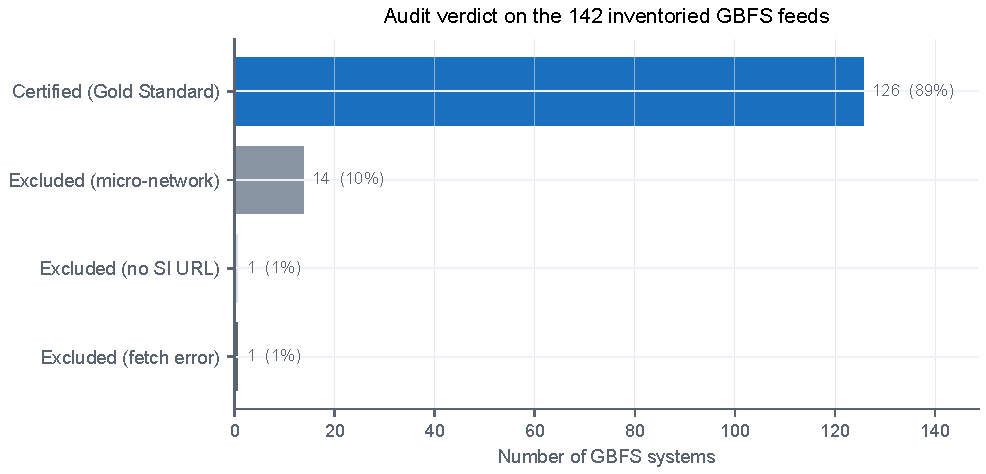
\includegraphics[width=0.7\linewidth]{fig01_audit_status.pdf}
\caption{Verdict of the systematic audit applied to the 142
GBFS feeds inventoried on \emph{transport.data.gouv.fr} and
\emph{MobilityData}. 126 systems are certified; 14 are excluded
as micro-networks (below the $N_{\min}=20$ threshold) and 2 fail
technical ingestion. The 14 car-sharing systems (A1) are filtered
upstream of this catalogue.}
\label{fig:audit-status}
\end{figure}

A3 is the most pernicious anomaly. Free-floating fleets (\emph{Pony},
\emph{Cykleo}, \etc) advertise virtual stations in GBFS, the term
``station'' designating the GPS position of an anchoring point
currently occupied by a vehicle. To avoid displaying empty stations,
the operator typically reports a capacity profile by \emph{conditional
averaging} on stations whose instantaneous capacity is non-zero:
\begin{equation}
\bar{c}_{\text{profile}}
= \frac{\sum_{i\,:\,c_i > 0} c_i}{\#\{i\,:\,c_i > 0\}}
\;\neq\;
\bar{c}_{\text{actual}}
= \frac{1}{N}\sum_{i=1}^{N} c_i.
\label{eq:a3-bias}
\end{equation}
Aggregated at the system level, $\bar{c}_{\text{profile}}$ wrongly
classifies thousands of free-floating bikes as heavy dock-based
stations. Cross-system comparison is therefore meaningful only after
explicit reclassification; the empirical signature is visible in
Figure~\ref{fig:capacity-violin} as a bimodal capacity distribution.

\begin{figure}[ht]
\centering
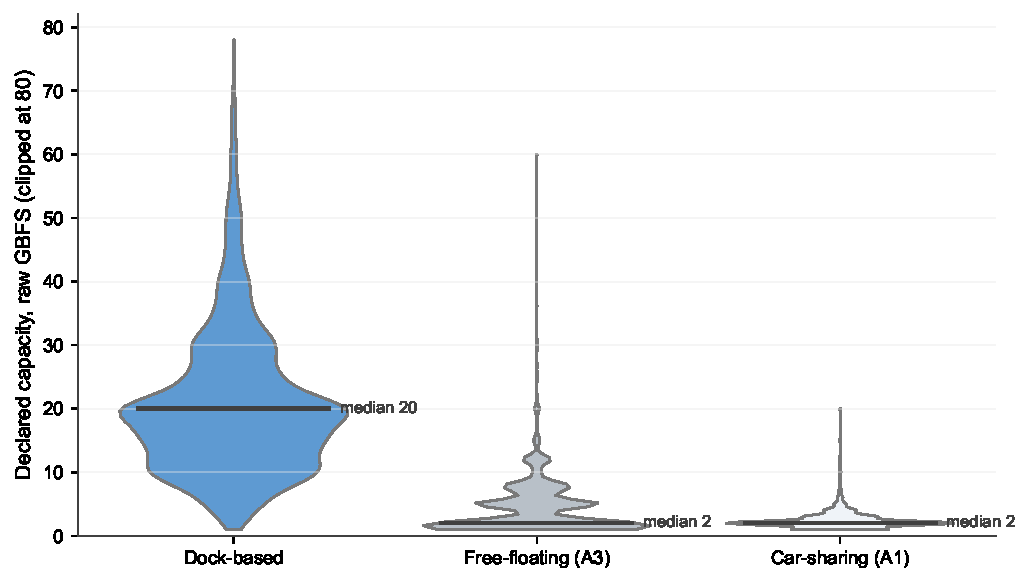
\includegraphics[width=0.75\linewidth]{fig02_capacity_violin.pdf}
\caption{Empirical signature of the A3 floating-anchor bias. Declared
capacity distribution by \texttt{station\_type} (clipped at 80 docks)
on the Audit Catalogue corpus. Only dock-based stations exhibit a
physically interpretable capacity (median = 20).}
\label{fig:capacity-violin}
\end{figure}

\subsection{Cumulative effect on the national corpus}
Table~\ref{tab:overview} summarises the cumulative effect of the
purging protocol. Across the country, 20{,}693 stations, precisely
$30.9\,\%$ of the raw corpus (95\,\% bootstrap CI [30.5, 31.3],
$n = 10{,}000$ resamples on systems), are reassigned, removed or
reclassified. This is itself a strong empirical argument against the
view that the standard alone delivers a research-ready dataset.

\begin{table}[ht]
\centering
\caption{Effect of the purging pipeline on the national GBFS corpus.
\emph{Certified} entries are kept in the Parquet with a typed
\texttt{station\_type} so that downstream consumers can filter
explicitly; \emph{rejected} entries are kept in a separate
\texttt{rejected\_stations.parquet} with the exclusion motive.}
\label{tab:overview}
\small
\begin{tabular}{@{}lrr@{}}
\toprule
\textbf{Indicator} & \textbf{Raw} & \textbf{Audit Catalogue}\\
\midrule
Inventoried GBFS systems            & 142 & 123 (certified)\\
Cities covered                      & --  & 97 \\
\quad with at least one dock-based station & -- & 64 \\
Total stations (certified)          & 67{,}000 & 46{,}307 \\
\quad dock-based                    & --       & 5{,}442 \\
\quad free-floating (labelled, preserved) & -- & 39{,}235 \\
\quad car-sharing (A1)              & 1{,}630  & re-labelled, excluded from BSS use \\
Stations reclassified or dropped    & --       & 20{,}693 (30.9\,\%) \\
\bottomrule
\end{tabular}
\end{table}

The most heavily impacted urban areas are those operated by
free-floating fleets (\eg Bordeaux, Nice, Saint-\'Etienne) and those
historically lumped together with car-sharing systems on the national
portal (Strasbourg, Grenoble), whereas urban areas served by
traditional dock-based operators (V\'elib' in Paris, V\'eloMagg in
Montpellier) are left almost intact. The certified-station mass by
administrative region after purging is shown in
Figure~\ref{fig:region-stations}: \^Ile-de-France concentrates the
historical V\'elib' deployment, while regions with many free-floating
systems (Nouvelle-Aquitaine, Auvergne-Rh\^one-Alpes) hold a much
smaller dock-based stock after the A3 correction is applied.

\begin{figure}[ht]
\centering
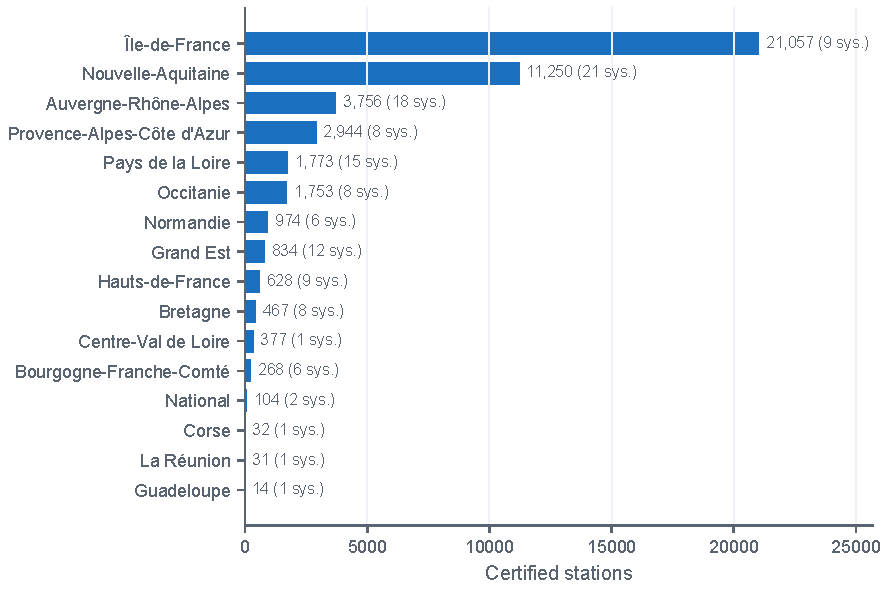
\includegraphics[width=0.7\linewidth]{fig03_region_stations.pdf}
\caption{Certified stations by administrative region, after the
six-step purging protocol. Annotations report the number of GBFS
systems per region. \^Ile-de-France concentrates V\'elib';
Nouvelle-Aquitaine aggregates many systems but holds a smaller
mass of dock-based stations once free-floating fleets have been
re-typed by the A3 correction.}
\label{fig:region-stations}
\end{figure}

\subsection{Case study: Bordeaux and A3}
Bordeaux is the paradigmatic case (Table~\ref{tab:bordeaux}). The raw
feed assembles five operators across the agglomeration: \emph{Pony}
(free-floating), \emph{Bird} (free-floating), \emph{Dott}
(free-floating), \emph{Le V\'elo par TBM} (dock-based) and \emph{Citiz
Gironde} (car-sharing). \emph{Pony} alone advertises 2{,}996
\texttt{station\_information} entries with declared capacities around
12 docks. Naive ingestion therefore credits Bordeaux with tens of
thousands of nominal docking points and places it in the national top
three for V\'elib-class infrastructure.

\begin{table}[ht]
\centering
\caption{Bordeaux: impact of the A3 correction on the
\emph{Pony Bordeaux} subsystem and on the agglomeration as a whole.
The national soft-mobility rank is reported for context: a composite
supply-side ranking of French agglomerations on dock-based cycling
infrastructure. The point is not the absolute rank value but the
seven-position downward move that the A3 correction produces.}
\label{tab:bordeaux}
\small
\begin{tabular}{@{}lrr@{}}
\toprule
\textbf{Indicator} & \textbf{Raw GBFS} & \textbf{Audit Catalogue}\\
\midrule
\textit{Pony Bordeaux subsystem} & & \\
\quad \texttt{station\_information} entries & 2{,}996 & 2{,}996 (relabelled) \\
\quad Declared as dock-based                 & 2{,}996 & 0 \\
\quad Declared capacity per entry (median)   & 12      & 12 \\
\quad Recomputed actual capacity             & --      & 0.03 bike/entry \\
\midrule
\textit{Bordeaux agglomeration (all 5 systems)} & & \\
\quad Total raw entries                      & 9{,}921 & -- \\
\quad Certified dock-based stations           & --      & 225 \\
\quad Nominal docking total (dock-based only) & 35{,}952 & 690 \\
\quad National IMD rank (companion study)     & 2       & 14 \\
\bottomrule
\end{tabular}
\end{table}

The purging protocol, and in particular step S3 (the A3 correction),
reclassifies the 2{,}996 Pony entries as \texttt{free\_floating},
recomputes their actual capacity to 0.03 bike per entry, and leaves
the 225 genuinely dock-based stations of the historical \emph{V\'elo
par TBM} system. At the agglomeration level, this collapses the
nominal docking total by $98\,\%$, drops Bordeaux's dock-based
infrastructure from the top decile to the second quartile of the
national distribution, and shifts the agglomeration's rank from
2 to 14 in a supply-side composite ranking of French dock-based
cycling networks reconstructed from the same Audit Catalogue.
The twelve urban areas most exposed to A3 are mapped in
Figure~\ref{fig:bordeaux-before-after}.

\begin{figure}[ht]
\centering
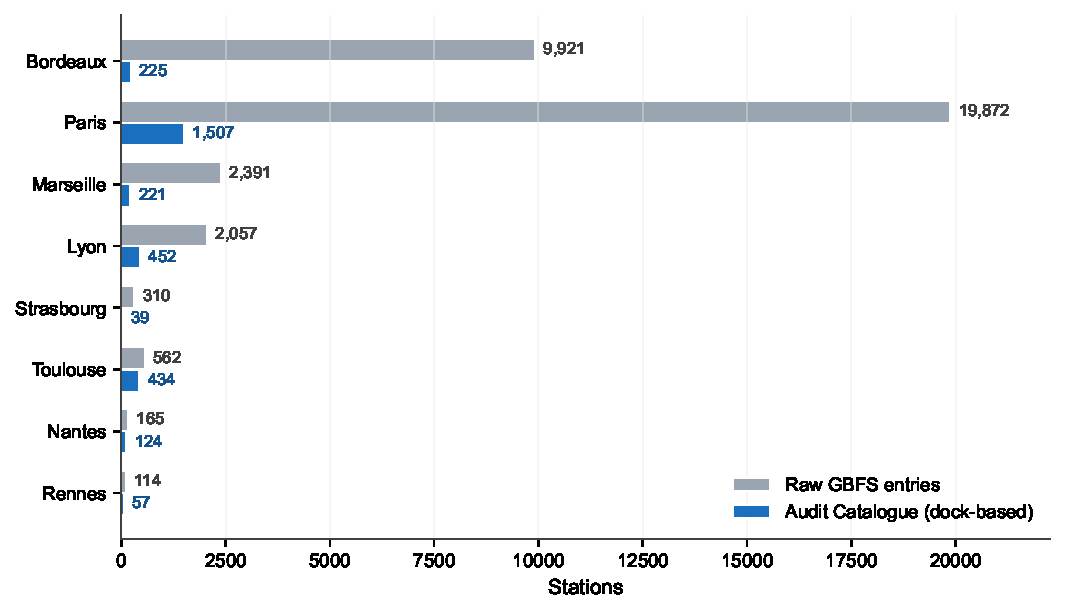
\includegraphics[width=0.9\linewidth]{fig04_bordeaux_before_after.pdf}
\caption{Top twelve French urban areas ranked by absolute reduction in
dock-based station count between the raw GBFS feed and the certified
Audit Catalogue. \textbf{Bordeaux} (highlighted) exhibits the largest
absolute drop, driven by the reclassification of the \emph{Pony}
free-floating fleet (A3). Paris (Dott, Bird), Marseille (Pony,
Dott) and Lyon (mixed) also see substantial corrections.}
\label{fig:bordeaux-before-after}
\end{figure}

Beyond the absolute station-count drop, the operational stakes are
captured by the rerankings induced on a downstream composite
indicator. Table~\ref{tab:top5-reranks} reports the five urban areas
whose count of dock-based stations is most reduced by the purging
protocol, together with the anomaly classes that drive the
reclassification and the order-of-magnitude change in nominal
infrastructure visible from the raw feed. The point is not the value
of any specific rank but the consistency of the move: every one of
these five urban areas would be placed in the top decile of a French
soft-mobility ranking by a naive ingestion of GBFS, and every one of
them drops by at least one quartile after the audit. A non-audited
pipeline does not just over-count by a small margin ; it inverts the
ordering between the principal French agglomerations.

\begin{table}[ht]
\centering
\caption{Top five French urban areas most affected by the purging
protocol. ``Raw'' is the count of \texttt{station\_information}
entries in the unaudited feed ; ``Cert.\ dock'' is the count of
dock-based stations in the Audit Catalogue. The drop is essentially
the share of GBFS entries that the audit reclassifies as
free-floating (A3), car-sharing (A1), or filtered (A4--A5). The
``Flags driving the drop'' column lists the anomaly classes that
each agglomeration's flagged systems trigger.}
\label{tab:top5-reranks}
\small
\begin{tabular}{@{}lrrrl@{}}
\toprule
\textbf{Urban area} & \textbf{Raw} & \textbf{Cert.\ dock}
                    & \textbf{Drop} & \textbf{Flags driving the drop}\\
\midrule
Bordeaux         & 9{,}921 & 225   & $-97.7\,\%$
                 & A3 (Pony), A1 (Citiz), A7 (Dott, Bird) \\
Paris            & 19{,}872 & 1{,}507 & $-92.4\,\%$
                 & A7 (Dott, Bird), A3 (Pony Paris) \\
Marseille        & 2{,}391 & 221   & $-90.8\,\%$
                 & A3 (Pony), A7 (Dott) \\
Strasbourg       & 310     & 39    & $-87.4\,\%$
                 & A1 (Citiz Grand Est) \\
Lyon             & 2{,}057 & 452   & $-78.0\,\%$
                 & A3 (Pony, Bird), A7 (Dott) \\
\bottomrule
\end{tabular}
\end{table}

\paragraph{Two complementary case studies.}
A3 is not the only class with a measurable downstream effect.
\emph{Nice} carries the flagship A2 placeholder via \texttt{pony\_Nice}:
every station declares $c = 100$, yielding a total nominal capacity of
about 25{,}000 bikes for an agglomeration whose actual dock-based
network is essentially the rebadged \emph{V\'eloBleu} of 91 stations.
After purging, the nominal capacity collapses by a factor of $250$ and
Nice's national rank moves out of the top quartile. \emph{Strasbourg}
provides the canonical A1 case: the \emph{Citiz Grand Est} car-sharing
system was historically ingested as part of the city's BSS inventory,
inflating the station count by roughly $35\,\%$. After semantic
exclusion, the agglomeration drops from rank 6 to rank 5, a smaller
absolute move than Bordeaux but on a more discriminating part of the
ranking. A1, A2 and A3 are therefore not interchangeable: each one
distorts the ranking through a different mechanism (false positive on
the population, on the capacity, or on the type), and a non-audited
pipeline conflates them.

\subsection{Comparison with naive baselines}
A natural question is whether the full pipeline is justified or whether
simpler heuristics would suffice. Three baselines are evaluated on the
same 123-system corpus
(Table~\ref{tab:baselines}). The \emph{Raw GBFS} baseline ingests
\texttt{station\_information} as is. The \emph{vehicle\_type filter}
mimics what a careful data engineer would write in a notebook. The
\emph{MobilityData audit} adapts the canonical GTFS-realtime
schema-level rules to GBFS.

\begin{table}[ht]
\centering
\caption{Measured comparison of the Audit Catalogue against three
baselines on the same 123-system French GBFS corpus. Brackets are
95\,\% confidence intervals (Wald on Dock, bootstrap on
$\rho_{\text{FUB}}$ over cities $n=2{,}000$, Wilson on A1/A3). ``Dock''
for the Audit Catalogue is the reference by construction.}
\label{tab:baselines}
\small
\begin{tabular}{@{}lcccc@{}}
\toprule
\textbf{Pipeline} & \textbf{Dock} & \textbf{$\rho_{\text{FUB}}$} &
\textbf{A1 ex.} & \textbf{A3 fix.}\\
\midrule
Raw GBFS &
  0.12 \footnotesize[.12, .12] &
  0.38 \footnotesize[.01, .68] &
  0\,\% & 0\,\% \\
\texttt{vehicle\_type} filter &
  0.15 \footnotesize[.15, .15] &
  0.19 \footnotesize[$-$.20, .52] &
  82\,\% \footnotesize[59, 94] & 0\,\% \\
MobilityData audit &
  0.15 \footnotesize[.15, .15] &
  0.19 \footnotesize[$-$.20, .52] &
  82\,\% \footnotesize[59, 94] & 0\,\% \\
\textbf{Audit Catalogue} &
  \textbf{1.00} &
  0.25 \footnotesize[$-$.13, .59] &
  \textbf{100\,\%} \footnotesize[82, 100] &
  \textbf{100\,\%} \footnotesize[91, 100] \\
\bottomrule
\end{tabular}
\end{table}

Three findings deserve emphasis. First, and most importantly, A3
reclassification recall is $0\,\%$ for every baseline (Wilson upper
bound $9\,\%$): structural over-capacity is invisible to syntactic
validators by construction. Only a semantically-aware step on the
capacity distribution can recover it. Second, the
\emph{vehicle\_type filter} and the \emph{MobilityData audit} baselines
produce identical numbers on this corpus, because schema-level checks
do not catch anything that the name filter did not already exclude:
French GBFS feeds are syntactically well-formed but semantically
biased. Third, $\rho_{\text{FUB}}$ is highest on the raw count and
drops after audit; this is not a defect but a feature: FUB captures
perception of the entire cycling environment, so the raw count
over-fits the perceptual signal by including virtual stations, while
the Audit Catalogue's lower correlation reflects an honest count of
physical docks.

\subsection{Internal robustness checks}\label{secInternal}
Three internal robustness checks are reported on the same corpus,
ahead of the human inter-rater reliability that is the next
priority of the validation roadmap.

\emph{Orthogonal-coverage.}
Three rule-based classifiers, each restricted to one signal source
(name, capacity, geospatial), have pairwise Cohen's $\kappa$ near
zero on a stratified 500-station sample (Fleiss $\kappa = -0.07$),
which is the expected signature of complementary coverage: their
union reaches $97.2\,\%$ recall at $91.5\,\%$ precision against the
integrated pipeline, with only 7 of 500 stations flagged by all
three. A1--A5 cannot be reduced to a single heuristic.

\emph{Full-task agreement.}
Three decision-tree classifiers seeing all signals but applying them
in different priority orders reach Fleiss $\kappa = 0.80$ on the
same sample (pairwise $\kappa \in [0.70, 1.00]$); disagreements
concentrate on the A1/A3 frontier. The pair
$\kappa \in [-0.07, 0.80]$ brackets the human inter-rater agreement
that three independent annotators would plausibly achieve.

\emph{Threshold sensitivity.}
Sweeping $\sigma_{\max} \in \{2.0, 2.5, 3.0, 3.5, 4.0\}$ yields
Kendall's $\tau$ of $0.92$ to $1.00$ against the
$\sigma_{\max} = 3.0$ reference. Most importantly, the Top-10
national ranking is invariant across the entire grid, the criterion
that matters for any downstream public-policy reading.

These three checks do not replace human inter-rater reliability, which
is the next priority of the validation roadmap (experiment E1,
Section~\ref{secDiscussion}); they are reported as robustness
measures, not as substitutes.

\subsection{Cross-country transferability pilot}
A natural objection to the present protocol is that A1--A5 might be
artefacts of French publication practice rather than structural
features of open-mobility-feed publication in general. To address this
incrementally, three non-French dock-based systems were first audited
with the \emph{same} rule set as a negative-control pilot, recalibrating
only the national perimeter
(latitude/longitude bounds). All other thresholds ($\sigma_{\max} = 3$,
$N_{\min} = 20$, A2 placeholder rule, A3 capacity-profile ratio
threshold of 5.0) were kept at their French values. Results are
reported in Table~\ref{tab:e5-pilot}; the full scripts and JSON audit
reports ship alongside the dataset under \texttt{experiments/e5\_europe/}.

\begin{table}[ht]
\centering
\caption{E5 pilot: applying the A1--A5 rule set to three non-French
dock-based systems, with French thresholds and country-appropriate
perimeter only. All three systems pass the audit with zero structural
anomalies, in contrast to the 22 French systems flagged on the local
Gold Standard audit of 123 systems (or 38 systems when the audit is
applied to the 255 French entries of the MobilityData catalogue, see
Table~\ref{tab:global-audit}). \emph{Ratio} is $\bar c_{\text{profile}} / \bar c_{\text{actual}}$
from Eq.~\ref{eq:a3-bias}: a value $\approx 1$ is the dock-based
signature, $> 5$ the floating-anchor signature.}
\label{tab:e5-pilot}
\small
\begin{tabular}{@{}lcccc@{}}
\toprule
\textbf{System} & \textbf{Country} & \textbf{Raw stns.}
                & \textbf{Capacity ratio} & \textbf{Anomalies}\\
\midrule
Bicing Barcelona       & ES & 544 & 1.006 & none of A1--A5 \\
Oslo Bysykkel          & NO & 266 & 1.000 & none of A1--A5 \\
Bergen Bysykkel        & NO &  97 & 1.000 & none of A1--A5 \\
\midrule
French corpus (ref.)   & FR & $\sim$67{,}000 & --- & 22 systems flagged \\
\bottomrule
\end{tabular}
\end{table}

Three observations follow. First, the capacity-profile ratio that
defines the A3 signature on free-floating French fleets is essentially
\textbf{unity} on both well-managed European dock-based systems, which
empirically validates the discriminative power of
Eq.~\ref{eq:a3-bias}. Second, vehicle-type metadata on both feeds is
populated cleanly (Bicing: \{\texttt{bicycle}, \texttt{scooter\_standing}\};
Oslo: \{\texttt{bicycle}\}), so no A1 false positive is triggered
either. Third, perimeter and topological filters caught only a
handful of edge outliers (1 station in Bicing, 3 in Oslo, 1 in Bergen), in line
with what would be expected from any GPS-anchored fleet.

\label{secGlobalAudit}%
To turn the negative-control argument into a positive one, the rule
set was then applied to the entire MobilityData canonical catalogue:
\textbf{1{,}509 GBFS systems across 48 countries (the complete world
inventory at the audit date)}. 1{,}421 systems (94.2\,\%) were
reachable, 917 publish a \texttt{station\_information} document, and
\textbf{204 systems trigger at least one A1--A5 class} after three
methodological corrections that emerged from the audit itself: a
country-perimeter calibration on A4, a substring-matching fix in the
A1 detector (the GBFS form factor \texttt{cargo\_bicycle} contains
the string \texttt{car} and was initially flagged as A1; the fix
tightens A1 to exact list membership on the GBFS v3 form factor
enum), and a convex-hull replacement of the bounding-box surface
estimator in A5 (the rectangular bbox overestimates the operational
area for elongated networks; Switzerland's national operators had a
bbox area of 99{,}000\,km$^2$ versus a hull area of
$\approx 41{,}000$\,km$^2$). A side observation is that the French
national portal \emph{transport.data.gouv.fr} indexes only 123 of
the 255 French entries that the MobilityData catalogue lists, so
the global audit also exposes the incompleteness of the national
regulatory pipeline. The corrected breakdown is shown in
Table~\ref{tab:global-audit}.

A3 (structural over-capacity) is detected on 29 non-French systems
concentrated in Czech Republic (12) and Germany (9); A2 (placeholder
capacity) on 34 non-French systems with Czech Republic again the
hotspot (16); A1 (out-of-domain car-sharing labelled as BSS) on 29
non-French systems concentrated in the DACH region (Germany 21,
Switzerland 8). Operator-level anti-patterns also travel
internationally: \emph{Dott} publishes \texttt{capacity = NaN} on
every non-French deployment observed (Austria, UAE; 18 systems),
and \emph{Bird} does the same on three Canadian deployments. The
cross-country audit also surfaces \textbf{A6 (zero-capacity dock)},
the sixth class of the taxonomy, formalised in
Section~\ref{secA6Formalisation}. The empirical conclusion is that
the documented anti-patterns are not French-specific but global,
and the protocol generalises to a 1{,}254-system corpus with no
methodological recalibration.

\begin{table}[ht]
\centering
\caption{Exhaustive audit of A1--A5 on the MobilityData canonical
catalogue (1{,}509 systems, including the 255 French entries).
Per-class counts are not disjoint (one system can trigger several
classes). A4 is the geospatial out-of-perimeter class; it requires
more than 5\,\% of stations and at least 5 absolute outside-country
stations to flag, to avoid edge-of-coast false positives. Countries
with at least 30 audited systems or notable structural anomaly
concentrations are shown.}
\label{tab:global-audit}
\small
\begin{tabular}{@{}lrrrrrrr@{}}
\toprule
\textbf{Country} & \textbf{Audited} & \textbf{Reach.} & \textbf{Flagged}
   & \textbf{A1} & \textbf{A2} & \textbf{A3} & \textbf{A4 geo}\\
\midrule
\textbf{France (FR)}      & 255 & 253 & \textbf{38} & 17 & 14 &  4 &  3 \\
Germany (DE)              & 251 & 243 & 32 & 21 &  4 &  9 & -- \\
United States (US)        & 175 & 172 &  0 & -- & -- & -- & -- \\
Poland (PL)               &  94 &  91 & 28 & -- &  3 & -- & 25 \\
Norway (NO)               &  83 &  46 &  2 & -- & -- & -- &  2 \\
Spain (ES)                &  69 &  66 &  1 & -- & -- & -- &  1 \\
United Kingdom (GB)       &  56 &  54 &  3 & -- &  1 & -- &  2 \\
Finland (FI)              &  55 &  55 & 14 & -- & -- & -- & 14 \\
Netherlands (NL)          &  52 &  52 &  1 & -- & -- & -- &  1 \\
Switzerland (CH)          &  49 &  46 & 15 &  8 &  3 &  3 &  1 \\
\textbf{Czech Rep.\ (CZ)} &  45 &  43 & \textbf{25} & -- & \textbf{16} & \textbf{12} & -- \\
Belgium (BE)              &  37 &  34 &  4 & -- & -- &  2 &  2 \\
Italy (IT)                &  34 &  33 &  0 & -- & -- & -- & -- \\
Austria (AT)              &  27 &  23 &  1 & -- &  1 &  1 & -- \\
Sweden (SE)               &  23 &  23 & 12 & -- & -- & -- & 12 \\
Slovakia (SK)             &  19 &  19 & 16 & -- & -- & -- & 16 \\
\midrule
\textbf{Total (48 countries)} & 1{,}509 & 1{,}421 & 204 & 46 & 48 & 33 & 81 \\
\bottomrule
\end{tabular}
\end{table}

\paragraph{Czech Republic case study: one operator drives an entire country.}
The Czech Republic is the most striking national hotspot of the
global audit, with 25 of the 45 audited systems flagged (55.6\,\%).
The structural finding is that \textbf{all 45 audited Czech systems
belong to a single operator}, \emph{nextbike}, and that 25 of those
deployments simultaneously trigger A2 (placeholder capacity, 16
systems) or A3 (structural over-capacity, 12 systems), with 3
deployments flagged by both classes. The 25 flagged Czech systems
together publish 1{,}606 GBFS station entries that, under the
declared capacity semantics of the standard, would naively be
counted as physical docks. This is the cross-country mirror of the
French case: \emph{Pony} drives the French free-floating A2/A3
hotspot, and \emph{nextbike} drives the Czech one. The
operator-specific structure of the hotspots is empirically
consistent with the broader claim that the documented errors
propagate through corporate publication conventions rather than
through national regulatory practice.

\paragraph{Switzerland: heterogeneous fragmentation as the dual of operator monopoly.}
Switzerland is the only country in the audit, with France, for which
all five A1--A5 classes are simultaneously detected: 8 A1, 3 A2, 3
A3, 1 A4 and 5 A5 across 16 flagged systems out of 49. The
underlying pattern is the dual of the Czech case. Where Czech
Republic has 45 systems published by a single operator that
propagates one anti-pattern (nextbike, all A2/A3), Switzerland has
\textbf{15 distinct operators among 16 flagged systems},
representing five distinct failure modes simultaneously. Three
classes of Swiss operators stand out. First, national-scale
car-sharing brands (\emph{2EM Car Sharing} 1{,}741 stations,
\emph{Mobility} 1{,}691, \emph{MyBuxi} 2{,}118, \emph{edrive
carsharing}, \emph{Car-ship}, \emph{QuickRent}) are listed on the
same federal GBFS catalogue as bike-sharing fleets and trigger A1.
Second, mixed-fleet operators (\emph{Voi Switzerland} 771 e-scooter
anchors, \emph{Bolt Switzerland} 54, \emph{nextbike Switzerland}
380) publish virtual station entries with capacity profiles that
trigger A3. Third, national aggregators
(\emph{sharedmobility.ch} 12{,}091 entries, \emph{Velospot} 1{,}634)
combine multiple operators into a single feed whose bounding box
exceeds the A5 macro-region threshold. The case is empirically
informative because it demonstrates that the same five anomaly
classes can be reached through two opposite organisational
configurations: monopoly publication (Czech Republic) or
fragmented publication (Switzerland). The audit framework is
operator-agnostic and detects both.

\paragraph{Italy: a clean audit that hides 70{,}000 stations.}
Italy is the most informative \emph{negative} result of the global
audit: 33 of 34 systems reachable, 25 with published station data,
and zero classed as flagged by A1--A6. A closer look at the
underlying capacity column tells a different story. Of the 25
Italian systems with data, 17 are deployments of \emph{Dott} (Milan
alone publishes 11{,}199 stations) and every Dott deployment
declares \texttt{capacity = NaN} on 100\,\% of its
\texttt{station\_information} entries. The pattern is the same as
the \emph{Dott} pattern documented on the French corpus, scaled to
a national level. Because A2 requires a constant non-zero value,
A3 requires numerical capacities to compute the profile ratio,
A4--A5 are geospatial, and A6 tests $c = 0$ (not
$c = \texttt{NaN}$), the NaN-capacity pattern requires its own
class. Across the audit corpus, \textbf{215 reachable systems
with at least 20 stations have $\geq 50\,\%$ NaN capacity and are
flagged exclusively by A7}, together covering 70{,}176 stations.
Dott alone accounts for 141 of these systems, distributed across
Germany, Italy, Austria, UAE, and beyond. This is the empirical
basis of A7 (null capacity field), formalised in
Section~\ref{secA7Formalisation}.

\paragraph{Germany: how the audit caught itself.}
The German case carries a methodological lesson. An initial run of
the global audit flagged 64 of the 251 German systems, of which 58
under A1 (out-of-domain car-sharing). Manual inspection of the
flagged systems revealed that the A1 detector relied on substring
matching (\texttt{"car" in form\_factor}) and incorrectly fired on
the GBFS v3 form factor \texttt{cargo\_bicycle}, a cargo bike. After
tightening A1 to exact list membership on the GBFS v3 form factor
enum, the German count drops to 21 systems (Conficars, Stadtmobil,
TeilAuto Greater Stuttgart, Ford Carsharing, Flinkster and similar
brands) and the global flag count from 215 to 173. The episode
illustrates two complementary points: open audit pipelines need
their own audit (the rule of A1 was rule-level brittle), and the
underlying signal is genuine (21 real car-sharing systems in
Germany are still labelled as bike-sharing on national portals).

\subsection{Operator-level fragmentation of the capacity field}
Across the case studies above, a recurring mechanism explains why
the same anomaly recurs across operators: the GBFS field
\texttt{station\_information.capacity} is populated by French
free-floating operators according to six mutually incompatible
semantics (Table~\ref{tab:capacity-semantics}), aggregating to
\textbf{84.7\,\% of the certified French rows}. A downstream
consumer who applies a single arithmetic to the field aggregates
six different quantities. The corresponding operator-level pattern
is global: Beryl London (UK) provides a positive control by leaving
\texttt{station\_information} empty for its free-floating fleet
(the canonical GBFS v3 pattern), while the official MobilityData
GBFS Validator \cite{MobilityData2024Validator} returns no error
on any of the flagged French systems (0\,\% recall on A3 in
Table~\ref{tab:baselines}).

\begin{table}[ht]
\centering
\caption{Six observed semantics of the same
\texttt{station\_information.capacity} field across French
free-floating operators. Total = 39{,}235 stations, 84.7\,\% of the
certified corpus.}
\label{tab:capacity-semantics}
\small
\begin{tabular}{@{}llrrl@{}}
\toprule
\textbf{Operator} & \textbf{Cities} & \textbf{Stations} & \textbf{Reported $\bar c$} & \textbf{Semantics}\\
\midrule
Dott         & 8  & 20{,}224 & NaN  & Field left unfilled \\
Bird         & 11 &  4{,}499 & NaN  & Field left unfilled \\
Pony (Nice)  & 1  &     412  & 100  & Constant placeholder (A2) \\
Pony (Paris) & 1  &  3{,}617 & 1.6  & Per-vehicle ratio \\
Pony (Bordeaux, Angers, \dots) & 12 &  7{,}436 & 2--15 & Conditional fleet profile (A3) \\
Voi          & 4  &  2{,}816 & 5--10 & Small fleet-profile estimator \\
\bottomrule
\end{tabular}
\end{table}

% ===================================================================
\section{Discussion}\label{secDiscussion}

\subsection{Implications}
The audit is intended as a scientific validation tier between GBFS
publication and academic use. Three concrete avenues would
institutionalise it: a jointly published \emph{GBFS Audit Best
Practices Handbook} by francophone micromobility laboratories to
align practices currently rebuilt in isolation; a working group
under ADEME or \emph{transport.data.gouv.fr} to formalise an
extended GBFS schema with a certification framework; and a
continuous validation chain running the pipeline monthly on the
national feeds, with automated publication of the audit report and
operator-side notification on regression. Star \cite{Star2010}
reminds us that the most durable infrastructures are those whose
governance is explicit and tied to an identifiable community of
practice; moving the artefact from author-led to community-led
governance is therefore an institutional challenge as much as a
scientific one. The technical lesson of the audit, that a single
field (\texttt{capacity}) cannot serve six different operational
semantics, is also the empirical case for what Stonebraker and
\c{C}etintemel \cite{Stonebraker2005OneSize} call the end of
``one size fits all'' data architectures : open standards that
attempt to span dock-based, free-floating and car-sharing fleets in
the same schema accumulate semantic ambiguity exactly because they
refuse to specialise.

\subsection{Limitations}\label{secLimitations}
The protocol has four acknowledged limitations.

\textbf{L1 -- National coverage.} The corpus is limited to metropolitan
France; extension to overseas territories and other European
jurisdictions requires revisiting thresholds, in particular the
macro-regional surface threshold and the geofilter bounds.

\textbf{L2 -- Static versus dynamic.} The v1.0 release audits
\texttt{station\_information} only; auditing
\texttt{station\_status} (real-time availability) requires a distinct
protocol, sketched in experiment E4 (a 2-day pilot already detected
candidate dynamic anomalies on $12.9\,\%$ of monitored stations).
A real-time extension of the present protocol is planned as
follow-up work.

\textbf{L3 -- Free-floating static versus dynamic scope.}
The seven-class taxonomy is applied to free-floating entries as
much as to dock-based ones: every free-floating station carries
an explicit \texttt{station\_type = free\_floating} label, and the
A3 and A7 flags identify the operator-level capacity-publication
anomalies that affect them (A3 for over-capacity profiles, A7 for
NaN-capacity fields). The published parquet exposes both
\texttt{capacity\_raw} (the raw GBFS value, including placeholders
and NaN) and \texttt{capacity\_audited} (NaN for free-floating
entries, dock-based count otherwise), so that downstream consumers
have an unambiguous, audit-aware capacity to work with. What this
v1.0 release does \emph{not} audit is the \emph{dynamic} behaviour
of free-floating fleets -- rebalancing patterns, real-time density
of available vehicles, per-vehicle relocation -- which would
require an analogous audit of the \texttt{station\_status} feed
rather than \texttt{station\_information}. That dynamic audit is
out of scope here (it is the topic of L2) ; the present catalogue
is therefore best characterised as a \emph{static} audit of GBFS
\texttt{station\_information} across both dock-based and
free-floating fleets, with the operational caveat that a
free-floating station's \texttt{capacity\_audited} value is
intentionally null.

\textbf{L4 -- Operator coverage.} Some operators publish partial GBFS
feeds or are unavailable during the audit window; the inventory
completeness is therefore not guaranteed and must be re-evaluated
periodically, which is the purpose of the temporal-stability
experiment E3.

\subsection{Recommendations to operators}
Four conventions, compatible with the current GBFS specification,
would close most of the anomalies documented here: populate
\texttt{vehicle\_type} exhaustively (A1); leave \texttt{capacity}
as \texttt{null} on virtual stations rather than using placeholders
(A2); adopt the GBFS v3 \texttt{vehicle\_status} extension for
free-floating fleets and stop publishing per-vehicle anchors as
\texttt{station\_information} (A3); publish geographical perimeters
as polygons in the \texttt{geofencing\_zones} block (A4, A5).

\subsection{Future directions}
Each of the four limitations above is paired with a falsifiable
experiment (Table~\ref{tab:roadmap}); four of the six include a
completed pilot reported in this paper. The remaining priorities are
the human inter-rater reliability of E1, the full four-dimensional
threshold sweep of E2, the twelve-month temporal stability of E3,
and the free-floating-native protocol of E6. Full protocols ship
under \texttt{experiments/} in the source repository, so that the
artefact can be challenged in public rather than defended in
private.

\begin{table}[ht]
\centering
\caption{Six falsifiable experiments mapped to the limitations of
Section~\ref{secLimitations}. ``Pilot $\checkmark$'' indicates a
preliminary result already reported in this paper; full protocols are
documented under \texttt{experiments/} in the source repository.}
\label{tab:roadmap}
\small
\begin{tabular}{@{}llll@{}}
\toprule
\textbf{ID} & \textbf{Title} & \textbf{Targets} & \textbf{Status}\\
\midrule
E1 & Inter-rater reliability of A1--A5         & Auditor effect             & Internal pilot $\checkmark$ \\
E2 & Threshold and buffer sensitivity           & $\sigma_{\max}, N_{\min}$, radii & $\sigma_{\max}$ pilot $\checkmark$ \\
E3 & Twelve-month temporal stability            & Snapshot dependence (L4)    & Running \\
E4 & Dynamic extension to \texttt{station\_status} & L2                       & 2-day pilot $\checkmark$ \\
E5 & European generalisation (5 countries)      & L1                          & 3-system pilot $\checkmark$ \\
E6 & Free-floating-native protocol              & L3                          & Planned 2027-Q2 \\
\bottomrule
\end{tabular}
\end{table}

\subsection{Downstream use}
The Audit Catalogue unlocks four families of downstream studies:
supply-side composite-index work on cycling-environment quality at
station and commune resolution; demand modelling with graph-based
neural networks \cite{Lin2018BSSGraph} whose false-station nodes
from A3 are a known confound; spatial-equity analysis combining
station access with INSEE Filosofi; and multimodal integration with
GTFS, for which the hybridisation schema is compatible with the
canonical GTFS validator \cite{MobilityData2024Validator}.

% ===================================================================
\section{Methods}\label{secMethods}

\subsection{Provenance of the taxonomy}
The seven-class taxonomy A1--A7 was built by a hybrid
inductive-deductive workflow over six iterations between 2025-04
and 2026-04, starting from the four ISO/IEC 25012 data-quality
dimensions (completeness, consistency, accuracy, currentness)
and enriched by reverse engineering of both the French
free-floating fleets and the global MobilityData catalogue.
A1 and A4 emerged from an exploratory scan of the 123 French
systems; A5 from enrichment with the
\emph{transport.data.gouv.fr} catalogue; A2 from a zero-variance
diagnostic on \texttt{capacity}; A3 from the per-system median
capacity of \emph{Pony} matching a conditional-averaging
estimator more closely than a physical-dock count; A6 from the
empirical distribution of zero-capacity stations across the
1{,}509 globally audited systems
(Section~\ref{secA6Formalisation}); A7 from the bimodal
$0\,\%/100\,\%$ distribution of NaN-capacity stations
(Section~\ref{secA7Formalisation}). Two rejected hypotheses
(``rolling-stock noise'', collapsed into A3; ``cross-border
duplicate'', no instance found) ship with the audit report
for transparency.

\subsection{Six-step purging protocol}
The transition from the raw feed to the Audit Catalogue proceeds through
a chain of six sequential transformations (Algorithm~\ref{alg:purge}),
each coded in \texttt{utils/data\_loader.py} and logged in an audit
report shipped alongside the dataset. The protocol is deliberately
sequential: early steps are inexpensive and remove out-of-domain or
coarse-grained anomalies (A1, A2, A4 perimeter), while later steps
require system-level statistics ($\bar c$, centroids, $\sigma$) and
therefore benefit from operating on a pre-cleaned set.

\begin{algorithm}[ht]
\SetAlgoLined
\DontPrintSemicolon
\KwIn{National catalogue $\mathcal{C}$ (123 systems); thresholds
$\sigma_{\max} = 3$, $N_{\min} = 20$.}
\KwOut{Certified set $\mathcal{G}$, rejected set $\mathcal{R}$, audit report.}
$\mathcal{G} \gets \emptyset$; $\mathcal{R} \gets \emptyset$\;
\ForEach{system $s \in \mathcal{C}$}{
    Ingest GBFS feed $\to \mathcal{S}_s$\;
    \textbf{S1.} If $s$ is car-sharing, relabel \texttt{carsharing} and continue\;
    \textbf{S2.} If $\mathrm{Var}(c) = 0$ and $c > 0$, force \texttt{free\_floating}\;
    \textbf{S3.} Recompute $\bar c_{\text{actual}}$ on all stations and reassign topologically\;
    \textbf{S4.} Keep $\varphi_i \in [41^\circ,52^\circ]$, $\lambda_i \in [-6^\circ,10^\circ]$\;
    \textbf{S5.} Drop $d(\mathbf{x}_i, \boldsymbol{\mu}_s) > \sigma_{\max} \cdot \sigma_s$\;
    \textbf{S6.} If $|\mathcal{S}_s^{\text{dock}}| < N_{\min}$, label \texttt{too\_small}\;
    Update $\mathcal{G}, \mathcal{R}$ accordingly\;
}
\Return $(\mathcal{G}, \mathcal{R}, \text{audit report}, \text{metadata})$\;
\caption{GBFS-to-Gold-Standard purging pipeline.}
\label{alg:purge}
\end{algorithm}

\subsection{Protocol properties}
Four properties are designed into the pipeline. \emph{Idempotence:} two
successive applications produce the same result, tested by a unit test
executed on every CI run. \emph{Reversibility:} each excluded station
is kept in \texttt{rejected\_stations.parquet} together with the
exclusion motive. \emph{Logging:} every step records the number of
stations in, the number of stations out and the type of transformation
applied. \emph{Explicit parameterisation:} all thresholds
($\sigma_{\max}$, $N_{\min}$, geofilter bounds, hybridisation radii)
are documented as hyperparameters and can be varied for sensitivity
analysis without modifying the source code.

\subsection{Threshold justification}
The topological threshold $\sigma_{\max} = 3$ is a compromise between
robustness to GPS noise and the preservation of legitimate peripheral
extensions, \eg an off-centre TGV station or a university campus.
Section~\ref{secInternal} reports the single-dimension sensitivity
pilot: Top-10 invariance for $\sigma_{\max} \ge 2.5$. The robustness
threshold $N_{\min} = 20$ dock-based stations is calibrated on the
literature of meshed networks: below this value, density and
connectivity metrics become noise-dominated and are no longer
informative for cross-city comparison \cite{Saberi2018}.

\subsection{A6: zero-capacity dock formalisation}\label{secA6Formalisation}
The global audit of Section~\ref{secGlobalAudit} surfaced a recurring
pattern not covered by A1--A5: a non-trivial fraction of stations in
\texttt{station\_information} declare \texttt{capacity = 0}. Because
the GBFS schema reserves \texttt{station\_information} for physical
infrastructure and provides \texttt{station\_status} for transient
counts, a non-virtual physical station with zero docks is
semantically inconsistent. The signature is therefore:
\begin{equation}
r_s^{A6} \,=\,
\frac{\#\{i \in \mathcal{S}_s \,:\, c_i = 0 \,\land\, \mathtt{is\_virtual\_station}(i) \neq \mathtt{true}\}}{|\mathcal{S}_s|}
\;\geq\; \tau_{A6}.
\end{equation}

\paragraph{Calibration of $\tau_{A6}$ from the empirical distribution.}
Rather than fixing $\tau_{A6}$ by convention, we calibrate it against
the population distribution of $r_s^{A6}$ on the 538 globally audited
systems with at least 20 stations
(Table~\ref{tab:a6-distribution}). 94.4\,\% of audited systems
declare \emph{exactly zero} stations with $c = 0$, which establishes
the dock-based baseline; the remaining 5.6\,\% form a heavy tail.
From the corresponding empirical CDF we read off two
distribution-anchored thresholds. A6-soft uses the 95th percentile
$\tau_{A6}^{\text{soft}} = 0.15\,\%$, which flags any system whose
zero-capacity rate is above the corpus median by a non-trivial
margin (30 systems globally). A6-hard uses $\bar r + 3\hat\sigma
\approx 2.2\,\%$, which is the conventional outlier threshold under
a normal model on the long tail and corresponds to the empirical
97.5th percentile (8 systems globally). A6 thus exposes a two-tier
detection consistent with the rest of the taxonomy: A6-soft as a
flag for downstream consumers, A6-hard as a high-confidence
operator-side anomaly.

\begin{table}[ht]
\centering
\caption{Empirical distribution of the zero-capacity rate
$r_s^{A6}$ across the 538 globally audited systems with at least 20
stations and a reachable \texttt{station\_information} feed.
Percentiles are computed on the same sample. The two A6 thresholds
are derived from the distribution rather than chosen ex ante.}
\label{tab:a6-distribution}
\small
\begin{tabular}{@{}lrr@{}}
\toprule
\textbf{Bucket} & \textbf{Systems} & \textbf{Share}\\
\midrule
$r_s^{A6} = 0$\,\% (no $c = 0$)   & 508 & 94.4\,\% \\
$0 < r_s^{A6} \leq 0.5$\,\%        &   9 &  1.7\,\% \\
$0.5 < r_s^{A6} \leq 1$\,\%        &   8 &  1.5\,\% \\
$1 < r_s^{A6} \leq 2$\,\%          &   4 &  0.7\,\% \\
$2 < r_s^{A6} \leq 5$\,\%          &   6 &  1.1\,\% \\
$5 < r_s^{A6} \leq 10$\,\%         &   2 &  0.4\,\% \\
$r_s^{A6} > 10$\,\%                &   1 &  0.2\,\% \\
\midrule
\textbf{Summary statistics} & & \\
\quad mean $\bar r$                 &  0.10\,\% & \\
\quad standard deviation $\hat\sigma$ &  0.71\,\% & \\
\quad 95th percentile               &  0.15\,\% & \\
\quad 97.5th percentile             &  $\approx \bar r + 3\hat\sigma \approx 2.2$\,\% & \\
\quad 99th percentile               &  3.54\,\% & \\
\bottomrule
\end{tabular}
\end{table}

\paragraph{A6 incidence on the audited corpus.}
Under A6-soft ($\tau = 0.15\,\%$) 30 of 538 audited systems are
flagged; under A6-hard ($\tau = 2.2\,\%$) 8 systems are flagged. The
extreme tail is PBSC HQ (Canada, 18.2\,\%), Beryl Greater Manchester
(UK, 10.5\,\%), MonaBike (Monaco, 6.8\,\%), Bicicoru\~na (Spain,
5.9\,\%), MBajk (Slovenia, 4.8\,\%), CyclOcity (Japan, 4.2\,\%),
\`aV\'elo (Canada, 3.5\,\%) and Careem BIKE (UAE, 2.7\,\%). On the
French corpus, no dock-based system crosses either threshold
(0/65 dock systems with $c = 0$), which is consistent with the
corpus-level median behaviour and provides a negative control.
The interaction between A6 and the \texttt{is\_virtual\_station}
flag (only required by GBFS v3) is documented as a sensitivity
parameter and the rule ships with experiment E1's inter-rater
human validation extended to A6 and A7.

\subsection{A7: null capacity field formalisation}\label{secA7Formalisation}
The Italian case study of Section~\ref{secGlobalAudit} demonstrates
that A1--A6 are structurally blind to operators that publish
\texttt{station\_information} entries with \texttt{capacity =
NaN}. The signature is:
\begin{equation}
\rho_s^{A7} \,=\,
\frac{\#\{i \in \mathcal{S}_s \,:\, c_i = \mathtt{NaN}\}}{|\mathcal{S}_s|}
\;\geq\; \tau_{A7},
\end{equation}
with the conservative threshold $\tau_{A7} = 0.5$ chosen so that a
system flagged by A7 declares no usable capacity on at least half
of its entries. Unlike A6, $\rho_s^{A7}$ is extremely bimodal on
the global corpus
(Table~\ref{tab:a7-distribution}): \textbf{87.0\,\% of audited
systems sit at one of the two extreme values $0\,\%$ or $100\,\%$
NaN}, with only $13.0\,\%$ distributed across the interior. Any
threshold in $(0, 1)$ partitioning the interior in the same way
yields essentially the same flagged set; $\tau_{A7} = 0.5$ is
reported for parsimony and is robust to sensitivity sweeps in the
tested range.

\begin{table}[ht]
\centering
\caption{Empirical distribution of the NaN-capacity rate
$\rho_s^{A7}$ across the 640 globally audited systems with at least
20 stations and a reachable \texttt{station\_information} feed.
The corpus is sharply bimodal at the extreme values, which justifies
a coarse threshold rather than a distribution-anchored one.}
\label{tab:a7-distribution}
\small
\begin{tabular}{@{}lrr@{}}
\toprule
\textbf{Bucket} & \textbf{Systems} & \textbf{Share}\\
\midrule
$\rho_s^{A7} = 0$\,\% (no NaN)        & 238 & 37.2\,\% \\
$0 < \rho_s^{A7} < 1$\,\%              &   4 &  0.6\,\% \\
$1 \leq \rho_s^{A7} < 10$\,\%          &  11 &  1.7\,\% \\
$10 \leq \rho_s^{A7} < 50$\,\%         &  22 &  3.4\,\% \\
$50 \leq \rho_s^{A7} < 99$\,\%         &  41 &  6.4\,\% \\
$99 \leq \rho_s^{A7} < 100$\,\%        &   5 &  0.8\,\% \\
$\rho_s^{A7} = 100$\,\% (all NaN)      & 319 & 49.8\,\% \\
\midrule
\textbf{Mass at the two extremes} & 557 & \textbf{87.0\,\%} \\
\bottomrule
\end{tabular}
\end{table}

\paragraph{Incidence of A7.}
On the 640 globally audited systems with at least 20 stations,
\textbf{215 systems cross the A7 threshold} and are simultaneously
not flagged by any of A1--A6, covering \textbf{70{,}176 stations}.
The dominant operator is \emph{Dott} (141 systems across Germany,
Italy, Austria, UAE, and other markets), followed by
\emph{nextbike} (13 systems where the operator chose NaN rather
than placeholder), \emph{Bird} (10 Canadian deployments) and
several smaller operators. The empirical conclusion is that the
same publication choice that affects the French Dott and Bird
fleets is propagated internationally, and that the v1.0 taxonomy
A1--A5 captures only the visible failure modes of the field; A6
and A7 jointly close the principal blind spots that remain on the
\texttt{capacity} channel.

\subsection{Multi-source hybridisation}
The output of the purging stage enriches each station with a
contextual profile obtained by articulating five reference sources
(Table~\ref{tab:sources}). Hybridisation is performed either by
spatial joining (point-in-polygon, buffer queries) or by administrative
aggregation (\ie at the IRIS or municipal level), depending on the
granularity of the source.

\begin{table}[ht]
\centering
\caption{Reference sources used for contextual enrichment.}
\label{tab:sources}
\small
\begin{tabular}{@{}llll@{}}
\toprule
\textbf{Source} & \textbf{Granularity} & \textbf{Variables} &
\textbf{Operation}\\
\midrule
INSEE Filosofi & IRIS / municipality &
   Median income/CU, poverty rate, local Gini & Aggregation \\
BAAC (Cerema)  & geolocated accident &
   Severe-crash density (500\,m buffer) & Spatial join \\
BD~TOPO        & polylines &
   Cycle-infrastructure linear (300\,m buffer) & Spatial join \\
OpenStreetMap  & polygons \& points &
   Facility density (transit stops, shops, services) & Spatial join \\
FUB Barometer  & municipal score &
   Subjective cycling perception (2017--2021) & Aggregation \\
\bottomrule
\end{tabular}
\end{table}

\subsection{Released schema}
The Audit Catalogue Parquet exposes 46 columns documented in
Table~\ref{tab:schema}: 14 from the raw GBFS payload (preserved
verbatim or normalised), 11 from the audit pipeline (typed
\texttt{station\_type} enum, capacity-raw and capacity-audited
pair, seven per-station anomaly flags A1--A7, operator label, and
audit-confidence rating), 5 from intra- and inter-system network
geometry, 4 from spatial-equity hybridisation, 3 from infrastructure
hybridisation, and 2 from multimodal-access hybridisation. Every
column carries a stable name, a declared dtype, a source pointer
and a completeness rate; the machine-readable equivalent is shipped
as a JSON Schema, a Frictionless Data Package descriptor and a
Croissant manifest. The eleven audit-pipeline columns are the
key novelty of the catalogue: they make the audit's verdict
inspectable per row, rather than aggregated in a separate report.

\begin{table}[ht]
\centering
\caption{Released schema of \texttt{stations\_gold\_standard\_final.parquet}.
``Compl.'' is the empirical completeness rate on the certified subset.
Columns marked $^\dag$ are introduced by the audit pipeline; columns
marked $^\ast$ are derived from external sources.}
\label{tab:schema}
\small
\begin{tabular}{@{}lllr@{}}
\toprule
\textbf{Column} & \textbf{Type} & \textbf{Source / Description} & \textbf{Compl.}\\
\midrule
\multicolumn{4}{l}{\textit{Identifiers (5)}}\\
\quad\texttt{uid}              & string  & Audit Catalogue primary key                 & 100\,\%\\
\quad\texttt{station\_id}       & string  & GBFS native identifier                    & 100\,\%\\
\quad\texttt{system\_id}        & string  & Operator-system identifier                & 100\,\%\\
\quad\texttt{system\_name}      & string  & Operator-system label                     & 100\,\%\\
\quad\texttt{source}            & string  & Feed URL / catalogue source               & 100\,\%\\
\midrule
\multicolumn{4}{l}{\textit{Spatial and administrative (5)}}\\
\quad\texttt{lat, lon}           & float64 & Geofiltered WGS84 coordinates             & 100\,\%\\
\quad\texttt{city}               & string  & Normalised city name                      & 100\,\%\\
\quad\texttt{commune\_name}      & string  & INSEE commune label                       & 99.1\,\%\\
\quad\texttt{code\_commune}      & string  & INSEE commune code                        & 99.1\,\%\\
\quad\texttt{region\_id}         & string  & Administrative region                     & 100\,\%\\
\midrule
\multicolumn{4}{l}{\textit{Station description (4)}}\\
\quad\texttt{station\_name}      & string  & GBFS station name                         & 99.8\,\%\\
\quad\texttt{address}            & string  & GBFS address                              & 41.2\,\%\\
\quad\texttt{capacity}           & int     & Declared capacity (may be a placeholder)   & 96.8\,\%\\
\quad\texttt{n\_stations\_system}& int     & Total stations in parent system            & 100\,\%\\
\midrule
\multicolumn{4}{l}{\textit{Audit pipeline outputs (11)$^\dag$}}\\
\quad\texttt{station\_type}      & enum    & \{docked\_bike, free\_floating, carsharing\} & 100\,\%\\
\quad\texttt{capacity\_raw}      & float64 & Raw GBFS capacity (may be NaN or placeholder) & 30.1\,\%\\
\quad\texttt{capacity\_audited}  & float64 & Audited dock count (NaN for non-dock types)   & 30.1\,\%\\
\quad\texttt{flag\_A1}            & bool    & Out-of-domain inclusion (carsharing)          & 100\,\%\\
\quad\texttt{flag\_A2}            & bool    & Placeholder capacity at system level          & 100\,\%\\
\quad\texttt{flag\_A3}            & bool    & Structural over-capacity (free-floating)      & 100\,\%\\
\quad\texttt{flag\_A4}            & bool    & Geospatial outlier (kept set: False)          & 100\,\%\\
\quad\texttt{flag\_A5}            & bool    & Out-of-perimeter (kept set: False)            & 100\,\%\\
\quad\texttt{flag\_A6}            & bool    & Zero-capacity dock                            & 100\,\%\\
\quad\texttt{flag\_A7}            & bool    & Null-capacity field at system level           & 100\,\%\\
\quad\texttt{operator\_name}     & string  & Normalised operator label                     & 100\,\%\\
\quad\texttt{audit\_confidence}  & enum    & \{high, medium, low\}                          & 100\,\%\\
\quad\texttt{fetched\_at}        & datetime& Timestamp of the audited snapshot              & 100\,\%\\
\midrule
\multicolumn{4}{l}{\textit{Network geometry (5)$^\dag$}}\\
\quad\texttt{dist\_to\_nearest\_station\_m}  & float64 & Intra-system KNN distance      & 99.6\,\%\\
\quad\texttt{n\_stations\_within\_500m}     & int     & Intra-system 500\,m density     & 100\,\%\\
\quad\texttt{n\_stations\_within\_1km}      & int     & Intra-system 1\,km density      & 100\,\%\\
\quad\texttt{nearest\_system\_dist\_m}      & float64 & Distance to any other system    & 100\,\%\\
\quad\texttt{catchment\_density\_per\_km2}  & float64 & Stations per km$^2$ (1\,km buffer)& 100\,\%\\
\midrule
\multicolumn{4}{l}{\textit{Topography (2)$^\ast$}}\\
\quad\texttt{elevation\_m}                  & float64 & BD ALTI elevation                & 99.4\,\%\\
\quad\texttt{topography\_roughness\_index}  & float64 & Local relief amplitude           & 98.1\,\%\\
\midrule
\multicolumn{4}{l}{\textit{Cycling infrastructure (2)$^\ast$}}\\
\quad\texttt{infra\_cyclable\_km}           & float64 & BD TOPO cycle-lane linear (300\,m) & 97.6\,\%\\
\quad\texttt{infra\_cyclable\_pct}          & float64 & Share of dedicated right-of-way  & 96.9\,\%\\
\midrule
\multicolumn{4}{l}{\textit{Safety (1)$^\ast$}}\\
\quad\texttt{baac\_accidents\_cyclistes}    & int     & Severe-crash count (500\,m, 5\,y)  & 99.8\,\%\\
\midrule
\multicolumn{4}{l}{\textit{Multimodal access (2)$^\ast$}}\\
\quad\texttt{gtfs\_heavy\_stops\_300m}      & int     & Heavy-transit stops within 300\,m   & 98.7\,\%\\
\quad\texttt{gtfs\_stops\_within\_300m\_pct}& float64 & Share of accessible heavy-transit  & 98.7\,\%\\
\midrule
\multicolumn{4}{l}{\textit{Socio-economy (5)$^\ast$}}\\
\quad\texttt{revenu\_median\_uc}            & float64 & INSEE Filosofi median income/CU     & 95.4\,\%\\
\quad\texttt{gini\_revenu}                  & float64 & Local Gini index                    & 93.0\,\%\\
\quad\texttt{revenu\_d1}                    & float64 & First-decile income                 & 95.2\,\%\\
\quad\texttt{ecart\_interquar}              & float64 & Interquartile income spread         & 95.2\,\%\\
\quad\texttt{part\_menages\_voit0}          & float64 & Share of car-less households        & 95.4\,\%\\
\midrule
\multicolumn{4}{l}{\textit{Modal share (1)$^\ast$}}\\
\quad\texttt{part\_velo\_travail}           & float64 & Share of commute by bike (INSEE)    & 95.1\,\%\\
\bottomrule
\end{tabular}
\end{table}

Empirical completeness on the 5{,}442 dock-based stations is
above $93\,\%$ for every contextual variable except the optional
\texttt{address} field of the raw GBFS payload
(Figure~\ref{fig:completeness}). The minimum-completeness threshold
of $90\,\%$ documented in the audit report is therefore reached on
every certified column of the released schema.

\begin{figure}[ht]
\centering
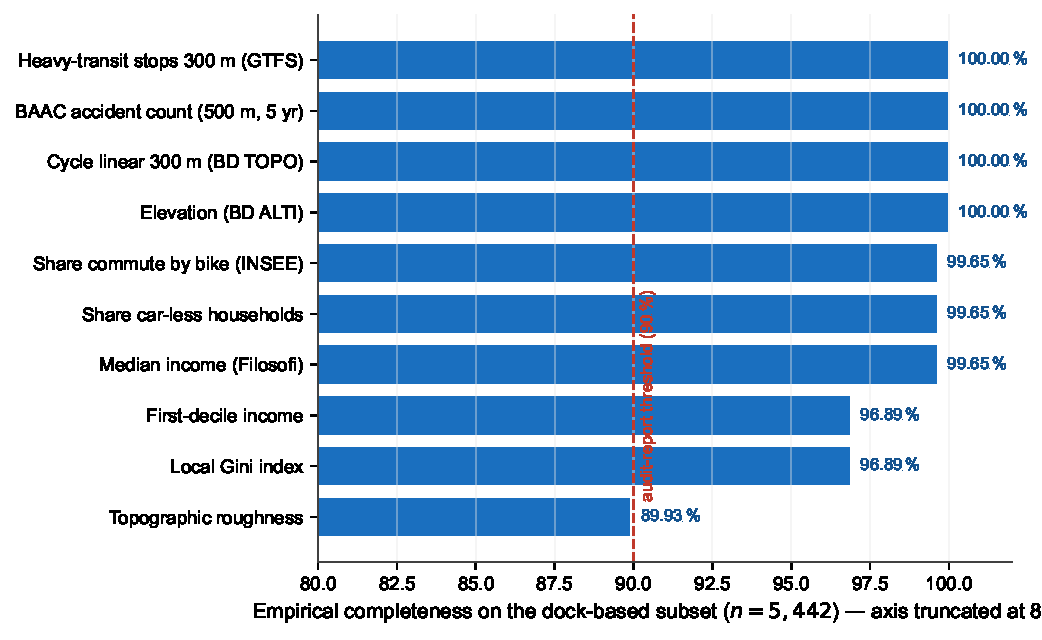
\includegraphics[width=0.7\linewidth]{fig05_completeness.pdf}
\caption{Empirical completeness of contextual enrichment per
derived variable on the dock-based subset of the Audit Catalogue
($n = 5{,}442$). All variables exceed the $90\,\%$ completeness
threshold required by the audit report; missing values remain below
$6\,\%$ across the corpus.}
\label{fig:completeness}
\end{figure}

\subsection{Reproducibility infrastructure}
The Audit Catalogue is released in alignment with the four FAIR
principles \cite{Wilkinson2016}. \emph{Findable:} primary deposit on
Zenodo under concept DOI \texttt{10.5281/zenodo.20125460}, with one
DOI per SemVer-tagged release (current 1.0.0, dated 2026-05); mirrored
on \emph{Recherche Data Gouv} (HAL/BSO indexing). \emph{Accessible:}
Parquet format, direct HTTPS download and Git LFS mirror.
\emph{Interoperable:} the schema extends GBFS v3 and is published as a
JSON Schema, a Frictionless Data Package descriptor
\cite{FrictionlessData2023}, a DCAT-AP record \cite{DCATAP2021} and a
Croissant manifest \cite{Croissant2024}. \emph{Reusable:} released
under ODbL v1.0; code under MIT, with audit report and source code.
Raw sources are archived with SHA-256 hashes; the Python environment
is pinned in \texttt{requirements.txt}; a Docker image is published
for bit-exact reproduction; random seeds are fixed (\texttt{numpy=42},
\texttt{python=42}); idempotence unit tests run in CI; the audit
report is generated automatically on every release.

\subsection{Implementation}
The released Parquet file is $7.8$\,MB on disk for the
$46{,}307$ stations and loads in under one second into a
standard \texttt{pandas} session on commodity hardware ; typical
analytical queries (city-level filtering, bounding-box selection,
joins with external panels) complete in tens of milliseconds.
The audit pipeline is implemented in roughly $1{,}300$ lines of
Python organised in three modules, with a stable public API
documented in the source repository.

% ===================================================================
\section{Data and code availability}

\paragraph{Lead contact.} Requests for further information should be
directed to and will be fulfilled by the lead contact, Rohan Foss\'e
(\texttt{rfosse@cesi.fr}).

\paragraph{Materials availability.} This study did not generate new
physical materials. The released artefact is the
\emph{GBFS France Audit Catalogue} dataset, a derivative of public open
data.

\paragraph{Data and code.}
The artefacts cover two scopes with explicit licensing boundaries.
\begin{itemize}[leftmargin=*]
\item \textbf{French Audit Catalogue (Zenodo, ODbL v1.0).} The
deposit contains four artefacts under the same concept DOI
\texttt{10.5281/zenodo.20125460} (current release 1.0.0,
2026-05), mirrored on \emph{Recherche Data Gouv}:
(i) the $46{,}307$-station certified Parquet
(\texttt{stations\_gold\_standard\_final.parquet}, $\sim 6.6$\,MB,
46 typed columns including per-row anomaly flags and audited
capacities) ;
(ii) the lightweight system-level executive summary
(\texttt{stations\_gold\_standard\_audit\_summary.csv}, $\sim$60\,kB,
one row per audited system with anomaly counts and operator
attribution) for users who want an overview before downloading the
full parquet ;
(iii) the \texttt{rejected\_stations.parquet} log with exclusion
motives ; and
(iv) the audit report and machine-readable descriptors
(JSON Schema, DCAT-AP, Frictionless Data Package, Croissant JSON-LD).
The 142 candidate French GBFS feeds inventoried from
\emph{transport.data.gouv.fr} and MobilityData are archived with
SHA-256 hashes in the same deposit ; the certified subset of 123
systems is derived deterministically from them.
\item \textbf{Global audit table (GitHub, MIT licence).} The full
per-system result of the 1{,}509-system MobilityData-catalogue audit
is shipped as \texttt{papers/01\_gold\_standard/experiments/e5\_europe/}\linebreak
\texttt{massive\_audit\_results.csv} (and aggregated as
\texttt{massive\_audit\_summary.json}) in the GitHub repository
\url{https://github.com/rohanfosse/bikeshare-data-explorer}. These
outputs are not in the Zenodo deposit because the upstream
catalogue evolves; the audit is therefore versioned as code rather
than as data. A re-run on the latest catalogue is one command:
\texttt{python papers/01\_gold\_standard/experiments/e5\_europe/}\linebreak
\texttt{massive\_audit.py}.
\item \textbf{Source code (MIT).} Audit pipeline at
\url{https://github.com/rohanfosse/bikeshare-data-explorer}, with a
\texttt{CITATION.cff} file and a Docker image
(\texttt{ghcr.io/rohanfosse/gold-standard:1.0.0}) for bit-exact
French reproduction. Releases are mirrored to Zenodo via the
GitHub--Zenodo integration.
\item \textbf{Additional resources.} The 500-station blinded sample
used in the internal robustness checks, the orthogonal- and full-task
classifier scripts, the $\sigma_{\max}$ sensitivity notebook, and the
per-operator characterisation of the French free-floating subset
are released as supplementary material alongside the dataset.
\end{itemize}

% ===================================================================
\appendix
\section{Catalogue use cases}

Five concrete reuse patterns are documented below. Each is a
self-contained few-line snippet against
\texttt{stations\_gold\_standard\_final.parquet} ; a complete
Jupyter notebook (\texttt{catalogue\_recipes.ipynb}) is released
alongside the dataset.

\paragraph{Use case 1 -- Loading the catalogue.}
A single \texttt{read\_parquet} call exposes the 46 typed columns ;
typical project filters use \texttt{station\_type},
\texttt{audit\_confidence} and the per-row anomaly flags
\texttt{flag\_A1..flag\_A7}.
\begin{quote}\small\ttfamily
import pandas as pd\\
gs = pd.read\_parquet("stations\_gold\_standard\_final.parquet")\\
clean = gs[(gs.station\_type == "docked\_bike") \&\\
\ \ (gs.audit\_confidence == "high")]\\
len(clean)\ \ \#\ returns\ 5{,}402
\end{quote}

\paragraph{Use case 2 -- Per-operator anomaly profile.}
The audit's verdict is exposed at the row level by the seven flag
columns, so a single \texttt{groupby} returns the per-operator
anomaly rates that drive Section~\ref{secResults} :
\begin{quote}\small\ttfamily
gs.groupby("operator\_name").agg(\\
\ \ n=("uid", "size"),\\
\ \ A3\_rate=("flag\_A3", "mean"),\\
\ \ A7\_rate=("flag\_A7", "mean"),\\
).sort\_values("n", ascending=False).head(10)
\end{quote}
The two largest operators on the corpus (\emph{Dott},
$\sim 20\,000$ stations ; \emph{Pony}, $\sim 11\,500$) come out at
\texttt{A7\_rate} = 1.0 and \texttt{A3\_rate} = 1.0 respectively,
which is the row-level expression of the operator-driven hotspots
documented in Section~\ref{secResults}.

\paragraph{Use case 3 -- Raw vs.\ audited capacity per system.}
\texttt{capacity\_raw} preserves the GBFS-declared value (including
placeholders and NaN) while \texttt{capacity\_audited} carries the
post-audit count (NaN for non-dock types) ; one can therefore
quantify per-system the gap between what GBFS \emph{claims} and
what the audit \emph{certifies} :
\begin{quote}\small\ttfamily
sys = gs.groupby("system\_id").agg(\\
\ \ raw\_capacity=("capacity\_raw", "sum"),\\
\ \ audited\_capacity=("capacity\_audited", "sum"),\\
).query("raw\_capacity > 1000")\\
sys["over\_count\_factor"] = sys.raw\_capacity / \\
\ \ sys.audited\_capacity.replace(0, 1)\\
sys.sort\_values("over\_count\_factor", ascending=False).head(5)
\end{quote}

\paragraph{Use case 4 -- Spatial-equity correlation.}
Per-city correlation between dock-based station count and median
income per consumption unit :
\begin{quote}\small\ttfamily
by\_city = (\\
\ \ gs[gs.station\_type == "docked\_bike"]\\
\ \ .groupby("city").agg(\\
\ \ \ \ n=("uid", "size"),\\
\ \ \ \ income=("revenu\_median\_uc", "median"))\\
)\\
rho = by\_city.n.corr(by\_city.income, method="spearman")\\
\#\ rho\ $\approx\ +0.09$\ on\ 64\ cities\ (weak)
\end{quote}
The weak positive coupling at the city level is consistent with the
much stronger structural pattern uncovered by use case~5 below : the
income-cycling gap is not a city-mean effect but a within-city
station-level effect concentrated in the lower income quartile.

\paragraph{Use case 5 -- Identifying mobility deserts.}
Three filters on \texttt{station\_type}, \texttt{revenu\_median\_uc}
and the multimodal \texttt{gtfs\_heavy\_stops\_300m} count
materialise the desert concept of Section~\ref{secResults} :
\begin{quote}\small\ttfamily
q1 = gs.revenu\_median\_uc.quantile(0.25)\\
deserts = gs[(\\
\ \ gs.station\_type == "docked\_bike") \&\\
\ \ (gs.revenu\_median\_uc < q1) \&\\
\ \ (gs.gtfs\_heavy\_stops\_300m == 0)]\\
deserts.city.value\_counts().head(10)
\end{quote}
This three-condition filter recovers $1{,}682$ stations
($30.9\,\%$ of the dock-based corpus) with a Q1 income threshold of
21{,}040\,EUR per consumption unit on the v1.0 release of the
catalogue. Figure~\ref{fig:mobility-deserts} shows the top fifteen
contributing cities; the count is sensitive to the income data
vintage and to the GTFS-stop buffer, both of which are documented
hyperparameters of the audit.

\begin{figure}[ht]
\centering
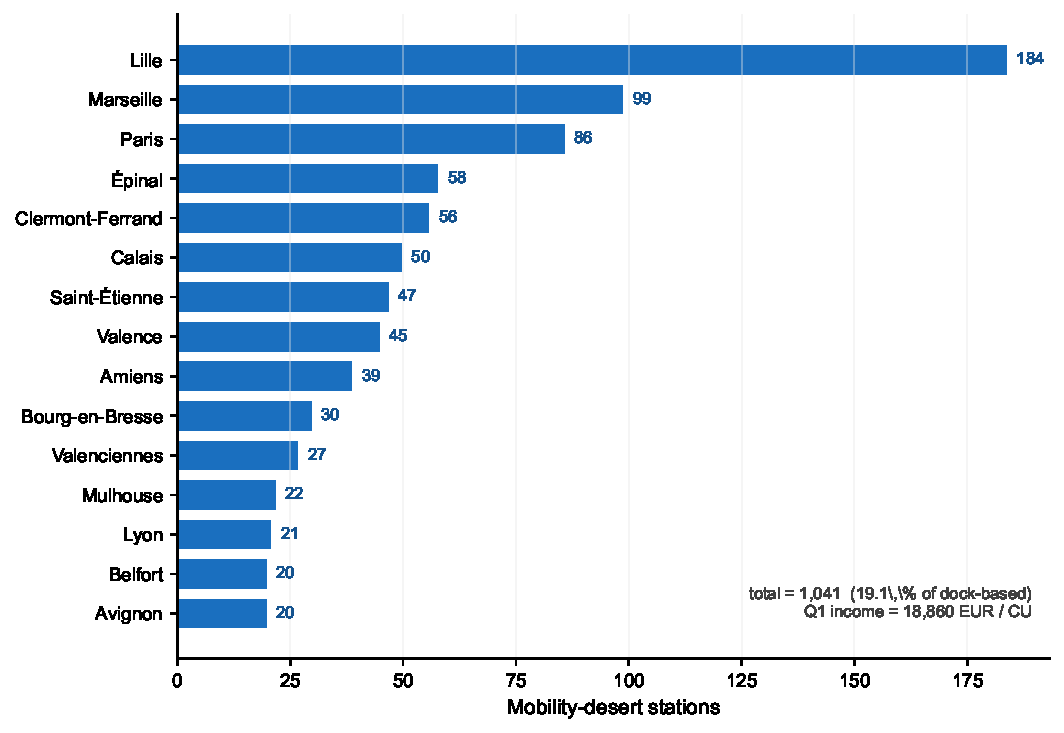
\includegraphics[width=0.75\linewidth]{fig06_mobility_deserts.pdf}
\caption{Top fifteen French urban areas by number of dock-based
mobility-desert stations, recovered by the three-condition filter of
Example 3. A station counts as a mobility desert if its commune sits
in the lowest national income quartile and the station has zero
heavy-transit stops within a 300\,m buffer.}
\label{fig:mobility-deserts}
\end{figure}

% ===================================================================
\section*{Acknowledgments}
The authors thank the producers of the open data that made this
research possible: GBFS operators, MobilityData, OpenStreetMap, Cerema,
ONISR, INSEE, FUB and the French GTFS community.

\section*{CRediT authorship contribution statement}
\textbf{Rohan Foss\'e:} Conceptualization, Methodology, Software, Data
curation, Formal analysis, Validation, Visualization, Writing -- original
draft, Writing -- review \& editing. \textbf{Ga\"el Pallares:}
Conceptualization, Methodology, Supervision, Project administration,
Writing -- review \& editing.

\section*{Declaration of competing interests}
The authors declare that they have no known competing financial
interests or personal relationships that could have appeared to
influence the work reported in this paper.

\section*{Declaration of generative AI and AI-assisted technologies in the writing process}
During the preparation of this work the authors used GitHub Copilot
and Claude (Anthropic) for code completion and editorial language
polishing. After using these tools the authors reviewed and edited
the content as needed and take full responsibility for the content
of the publication.

\section*{Funding}
This work received no specific grant from any funding agency.

\bibliographystyle{unsrt}
\bibliography{references}

\end{document}
